\documentclass[oneside, 12pt]{book}
\usepackage{icdthesisUTF}
\usepackage{tabularx} 
\usepackage{epsfig}

\renewcommand{\thesistitle}{Ανάπτυξη eργαλείου για την σχεδίαση παιχνιδιών με την βοήθεια υπο-λογιστή }
\renewcommand{\thesisauthor}{Γιώργου Μιχαηλίδη}
\renewcommand{\thesisauthorabbrv}{Γ. Μιχαηλίδης}
\renewcommand{\thesisauthorinitials}{ΓΜ}
\renewcommand{\thesissupervisor}{Δρ. Νικόλαος Πεταλίδης. Επιστημονικός Συνεργάτης}
\renewcommand{\thesismonth}{Φεβρουάριος}
\renewcommand{\thesisyear}{2016}

% Η βιβλιογραφία
\addbibresource{testUTF.bib}

\begin{document}
	
	\Titlepage
	\Declarationpage
	
	\begin{Abstract}
		Τα πρώτα ηλεκτρονικά παιχνίδια είχαν γραφτεί εξ'ολοκλήρου σε υλισμικό. Από τότε, οι κάρτες γραφικών και οι μικροεπεξεργαστές βελτιώθηκαν, δημιουργήθηκαν κονσόλες φτιαγμένες αποκλειστικά για ηλεκτρονικά παιχνίδια, με ειδικά χειριστήρια τα οποία σου προσφέρουν διαφορετικές εμπειρίες.
		Η διαδικασία ανάπτυξης λογισμικού είναι ακριβή και ο σχεδιασμός γίνεται όλο πιο σύνθετος και περίπλοκος. Τα έργα γίνονται όλο πιο απαιτητικά και δαπανηρά. Δημιουργήθηκε η ανάγκη για ένα εργαλείο το οποίο να παρέχει ένα ομοιογενές περιβάλλον για την ανάπτυξη σύνθετων έργων. 
		Ένα CASE (Computer Aided Software Engineering) tool είναι ένα λογισμικό-εργαλείο το οποίο απλοποιεί τον κύκλο ανάπτυξης ενός λογισμικού. 
		Στο τομέα του σχεδιασμού παιχνιδιών το πιο διαδεδομένο CASE tool είναι η μηχανή γραφικών. Μια μηχανή γραφικών είναι μια σουίτα από επαναχρησιμοποιήσιμα οπτικά εργαλεία τα οποία βρίσκονται σε ένα ενιαίο περιβάλλον.
		Σκοπός της πτυχιακής είναι να αναγνωριστούν μοτίβα και τεχνικές δημιουργίας παιχνιδιών, ώστε να δημιουργηθεί ένα εργαλείο το οποίο να το προσεγγίζει από υψηλό επίπεδο με αφαιρέσεις για εύκολη μοντελοποίηση και αυτοματοποίηση κατά τη δημιουργία.
	\end{Abstract}
	\tableofcontents
	\listoftables
	\listoffigures
	
	\begin{Preface}
		Εδώ μπορεί να μπει πρόλογος. (Δεν είναι απαραίτητο).
	\end{Preface}
	
	\begin{Acknowledgement}
		Ευχαριστίες (στο μπαμπά, στη μαμά, κτλ)
	\end{Acknowledgement}
	
	\begin{Definitions}
		Ορισμοί εννοιών που μπορεί να είναι χρήσιμοι. Για παράδειγμα:	
		\begin{description}
			\item [\LaTeX] Σύστημα στοιχειοθεσίας κειμένων
		\end{description}
		
	\end{Definitions}
	
	\chapter{Εισαγωγή}
			
		\leftmark\rightmark
		\section{Η τυπογραφία σήμερα}
		Αυτή είναι η αναφορά σε ένα άρθρο περιοδικού:\citep{Schmidt98}.Αυτή
		είναι η αναφορά σε ένα βιβλίο:\citep{goosens93}. Αυτή είναι η αναφορά
		σε ένα ελληνικό βιβλίο:\citep{Chatzigeorgiou05}. Βιβλίο στα ελληνικά
		με ξένο συγγραφέα:\citep{Sommerville09}. Άρθρο σε
		συνέδριο~\citep{4343930}. 
		
		Τέλος αναφορά σε ιστοσελίδα:~\citep{Wikipedia_BibTeX}.
		
		Εδώ αναφερόμαστε στo σχήμα~\ref{fig:image1}:
		\begin{figure}[h]
			\centering
			
\includegraphics[width=35mm]{lion.png}
			\caption{Παράδειγμα εικόνας}
			\label{fig:image1}
		\end{figure}
		
		και εδώ στον πίνακα~\ref{tab:table1}:
		\begin{table}[h]
			\centering
			\caption{Παράδειγμα πίνακα}
			\begin{tabularx}{\linewidth}[h]{|XXX|}%
				\hline
				\hline
				Κίνητρα & Παραδείγματα ευρημάτων & Αριθμός μελετών\\
				\hline
				Ταύτιση με το έργο & Ξεκάθαροι στόχοι &20\\
				Καλό management & Ομαδικότητα &16\\
				Συμμετοχή υπαλλήλων & Συμμετοχή στις αποφάσεις&16\\
				Προοπτικές εξέλιξης & Προοπτικές προαγωγής&15\\
				Ποικιλία στην εργασία & Καλή χρήση ικανοτήτων& 14\\
				Αίσθηση του να ανήκεις κάπου& Υποστηρικτικές σχέσεις&14\\
				Αμοιβές και κίνητρα & Αυξημένος μισθός& 14\\
				\hline
				\hline
			\end{tabularx}
			\label{tab:table1}
		\end{table}
		\appendix
	
		
	\chapter{Μηχανές γραφικών}
	
	\chapter{Διαδικτύωση}
		Διαδικτύωση στα ηλεκτρονικά παιχνίδια έχουμε όταν περισσότεροι από ένας παίχτες σε διαφορετικές πλατφόρμες ή υπολογιστές, μοιράζονται και αλληλεπιδρούν στο ίδιο εικονικό περιβάλλον. 
		
		\subsection{Το πρόβλημα}
		\paragraph{Περιγραφή του προβλήματος}
		Διάφοροι παίχτες σε διάφορα σημεία του πλανήτη θέλουν να μοιραστούν ένα εικονικό περιβάλλον σε πραγματικό χρόνο με σκοπό την συνεργασία ή αντιπαλότητα. O κόσμος είναι ένα υπερσύνολο του offline κόσμου με επιπλέων στοιχεία κοινωνικοποίησης όπως η επικοινωνία μέσω μηνυμάτων ή φωνής.
		
		\paragraph{Κατανόηση του προβλήματος}
		
		Ένας εικονικός κόσμος, περιλαμβάνει πολλές οντότητες οι οποίες αλληλεπιδρούν μεταξύ τους μέσω των μηχανισμών, νόμων και κανόνων που διέπουν τον κόσμο. Παράδειγμα μηχανισμού είναι η προσομοίωση του φυσικού κόσμου, όπου οι οντότητες αναποκρίνονται σε νόμους της φυσικής.
		
	    Κατά την ενημέρωση του κόσμου, ο προσομοιωτής χρησιμοποιώντας  τους νόμους, τους κανόνες και τους μηχανισμούς που διέπουν τον κόσμο, παίρνει ως είσοδο τις οντότητες και τα ειδικά βάρη των ιδιοτήτων τους, την απόλυτη θέση τους στο σύστημα συντεταγμένων του κόσμου, και το χρονικό διάστημα της προσομοίωσης και αναλύει την προσομοίωση. Η ανάλυση της προσομοίωσης για να είναι επιτρεπτά ακριβής πρέπει να γίνεται περίπου 80-100 φορές το δευτερόλεπτο. [αναφορά σε πηγή]
		
		Στο τέλος της προσομοίωσης, η μηχανή γραφικών αποτυπώνει τον κόσμο στις εξόδους με αναφορές σε στατικά assets, σε αλγόριθμους παραγωγής δυναμικών assets για την αναπαράσταση του κόσμου.
	
		\paragraph{Εξαγωγή απαιτήσεων}	
		Με βάση το πρόβλημα καταλήγουμε στο παρακάτω διάγραμμα ακολουθίας.
		
		\begin{figure}[h]
			\centering
			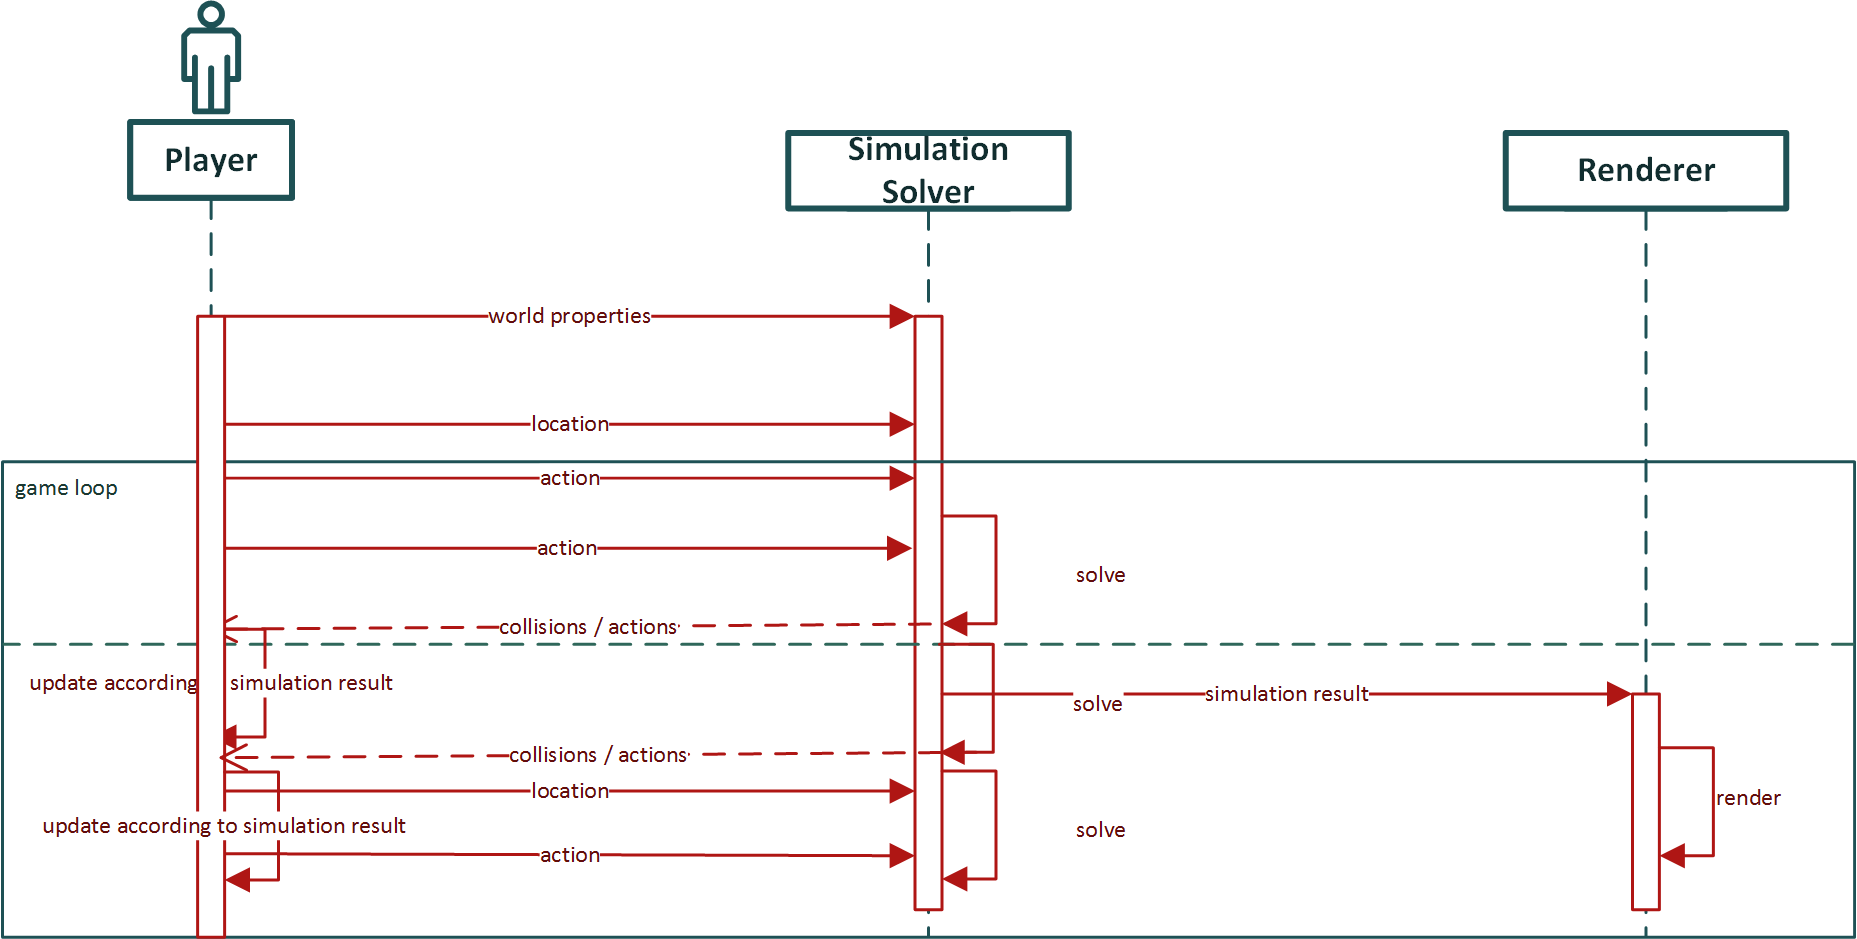
\includegraphics[width=100mm]{Images/gameloop_network_sequence}
			\caption{Network Sequence}
			\label{fig:Network Sequence}
		\end{figure}		
		
		Βλέποντας το διάγραμμα καταλαβαίνουμε ότι σε η διαδικασία rendering περιλαμβάνει στατικά στοιχεία και αλγόριθμους, τα οποίοι μπορούν να φορτώνονται τοπικά στον κάθε υπολογιστή, και δεν είναι απαραίτητα για την επίλυση της προσομοίωσης. Τα απαραίτητα στοιχεία για την προσομοίωση τα οποία πρέπει να μοιράζονται μεταξύ των παιχτών είναι:
		\begin{itemize}
			\item Oι ιδιότητες της οντότητας με βάση τους νόμους του κόσμου. Οι ιδιότητες αυτές δεν ενημερώνονται συχνά.
			\item Οι αλλαγές στο σύστημα συντεταγμένων και οι διάφορες ενέργειες της κατευθυνόμενης οντότητας κατά την πάροδο του χρόνου. Οι αλλαγές τοποθεσίας και ενέργειες γίνονται πολλές φορές ανά δευτερόλεπτο. Η προσομοίωση για να είναι ακριβής πρέπει να ενημερώνεται για τις διάφορες ενέργειες σε πραγματικό χρόνο.
		\end{itemize}
				
		\subsection{Εκπόνηση σχεδίου}	
		Η ανάγκη αποστολής πολλών μηνυμάτων ανά δευτερόλεπτο οδηγεί στη χρήση των network sockets. Τα sockets χρησιμοποιωντας ένα IP και  Port και επιτρέπουν την αποστολή και παραλαβή μηνυμάτων με βάση κάποιου πρωτόκολλου.
		
		\paragraph{Επιλογή πρωτοκόλου}
		\begin{itemize}	
			\item TCP: Το TCP (transmission control protocol), είναι το πιο συχνά χρησιμοποιημένο πρωτόκολλο. Η διασύνδεση με TCP είναι αξιόπιστη και τα μηνύματα παραλαμβάνονται στη σειρά αποστολής. Η αξιοπιστία όμως έρχεται με ένα μικρό κόστος απόδοσης.
			\item UDP: Το UDP (user diagram protocol) δεν περιλαμβάνει την αξιοπιστία και την εγγύηση της αλληλουχίας μηνυμάτων. Η απουσία λειτουργιών όμως, το κάνει το πιο γρήγορο σε αποστολή μηνυμάτων πρωτόκολλο.
			
			Η επιλογή πρωτοκόλλου γίνεται ανάλογα με το γενικότερο πλαίσιο και τη συγκεκριμένη χρήση του πακέτου αποστολής. Στην αποστολή της τοποθεσίας, το οποίο γίνεται 20φορές / δευτερόλεπτο, η αξιοπιστία δεν είναι το βασικότερο, αλλά η απόδοση. Στην αποστολή των στοιχειών του χρήστη κατά την έναρξη, ή ενώς γραπτού μηνύματος πρέπει να είναι αξιόπιστη.
		\end{itemize}

		\paragraph{Επιλογή αρχιτεκτονικής δικτύου}
			Οι αρχιτεκτονικές δικτύου χωρίζονται ανάλογα με το που γίνεται η επίλυση και επεξεργασία της προσομοίωσης.  
		\begin{itemize}	
			\item Client-server model: στο οποίο ο client απλά κάνει render και το μεγαλύτερο κομμάτι της λογικής και της προσωμοίωσης τρέχει στον server. Ο server στέλνει οδηγίες στον client για το τι να κάνει render και ο client απλά υπακούει.
			\item Client on top of server model: ο client είναι και server, δηλαδή οι μηχανές που έχουν τον client έχουν και τον server.
			\item Peer-to-peer: οι μηχανές συμπεριφέρονται μερικώς ως clients και μερικώς ως servers, δηλαδή έχουν και στοιχεία λογικής και επεξεργασίας.
		\end{itemize}
			Η client-server αρχιτεκτονική εφαρμόζεται σε παιχνίδια τα οποία περιλαμβάνουν πολύ μεγάλους κόσμους και η προσομοίωση περιλαμβάνει αλληλεπιδράσεις μεταξύ πολλών οντοτήτων. Οι προσωμοιώσεις αυτές γίνονται σε εξειδικευμένες μηχανές και όχι στον προσωπικό υπολογιστή του κάθε χρήστη γιατί χρειάζονται μεγάλους υπολογιστικούς πόρους. Επίσης ο server μπορεί να λύσει race conditions και να λειτουργήσει ως "διαιτητής" μεταξύ δύο οντοτήτων οι οποίες ζητούν πρόσβαση στο ίδιο σύστημα κατά το ίδιο χρονικό διάστημα. Οι αρχιτεκτονικές στις οποίες ο client περιλαμβάνει στοιχεία επεξεργασίας του κοινόχρηστου κόσμου, είναι πιο δύσκολες στην ανάπτυξη συντήρηση γιατί δημιουργούνται race conditions στο χρονικό διάστημα αποστολής-παραλαβής μηνυμάτων που προορίζονται σε αλληλοεξαρτώμενες λειτουργίες.
			
		\subsection{Σχεδίαση του framework}
		\paragraph{Φάσεις}
		
		\subsection{Αρχιτεκτονική}		
			\begin{figure}[h]
				\centering
				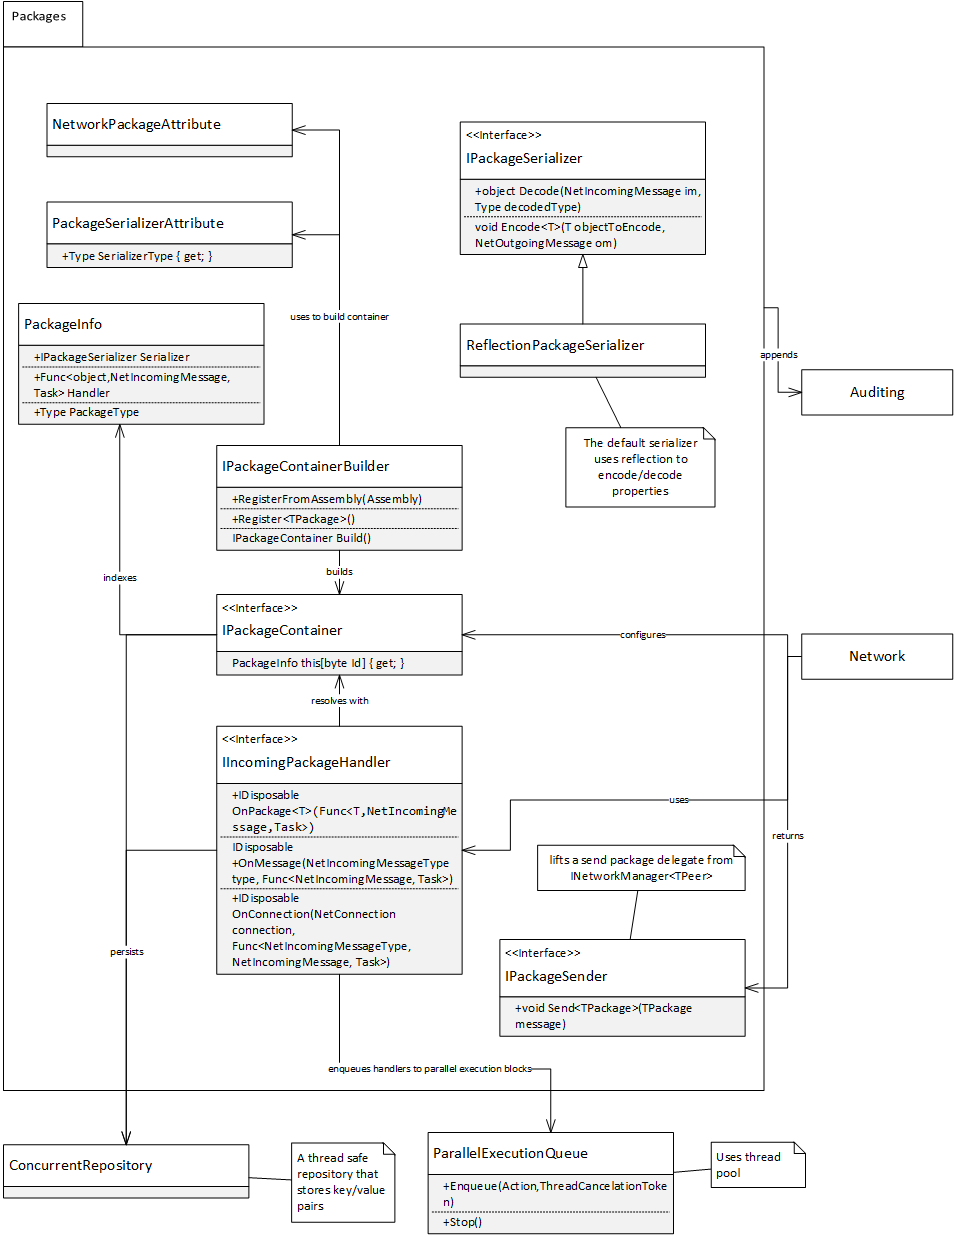
\includegraphics[width=165mm]{Images/network_architecture_packages}
				\caption{Network Packages Module}
				\label{network_packages}
			\end{figure}
			
			
			
			\subsection{Ανταλλαγή μηνυμάτων}
			
			\subsection{Client}	
			
			\subsection{Server}	

	\chapter{Game Host}
	\section{Αρχιτεκτονική}		
	
	\chapter{Περίληψη}
	
	\begin{Glossary}
		Το γλωσσάρι μπορεί να είναι χρήσιμο αν χρησιμοποιείτε πολλά ακρώνυμα
		και συντομογραφίες. Για παράδειγμα
		\begin{description}
			\item[TCP]Transmission Control Protocol
		\end{description}
	\end{Glossary}
	
	\printbibliography
	%\lastpageinfo
	




\end{document}
